\documentclass{beamer}

%Russian-specific stuff
\usepackage[T2A]{fontenc}
\usepackage[utf8]{inputenc}

\usepackage{hyphenat}
\hyphenation{ма-те-ма-ти-ка}
%end of Russian-specific packages

\usepackage{graphicx}
%\usepackage{subfigure}
\usepackage{subcaption}

\title{Микроквазары}
\subtitle{МФК `Космические тайны рентгеновского неба'}
\titlegraphic{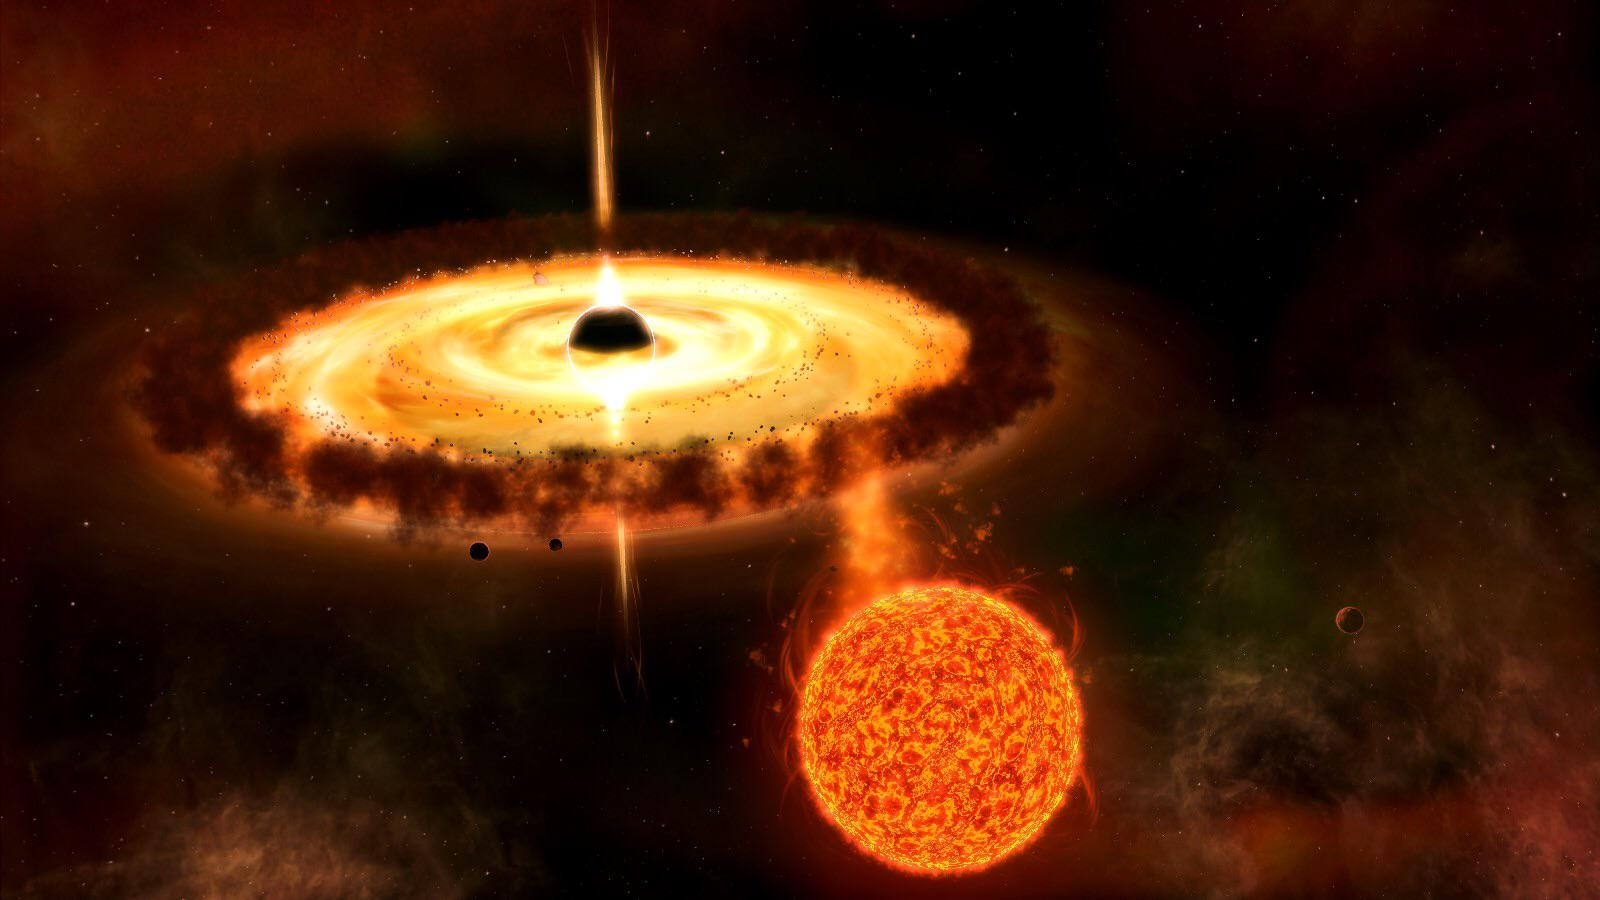
\includegraphics[width=.6\textwidth]{resources/microquasar-stellaris.jpg}}
\author{Фельдшеров Сергей}
\date{20 Апреля 2022}
%\date{}

\begin{document}

%\maketitle

\begin{frame}
	\titlepage
\end{frame}

\begin{frame}
	\frametitle{Ярчайшие объекты во вселенной}
	Квазары (\textbf{quas}i-stell\textbf{ar r}adio source) - невероятно яркие активные ядра
	галактик, состоящие из:
	\begin{itemize}
		\item сверхмассивной чёрной дыры
		\item окружающего аккреционного диска
	\end{itemize}
	Излучение исходит от разогретого трением вещества аккреционного диска.
	\begin{figure}[h]
		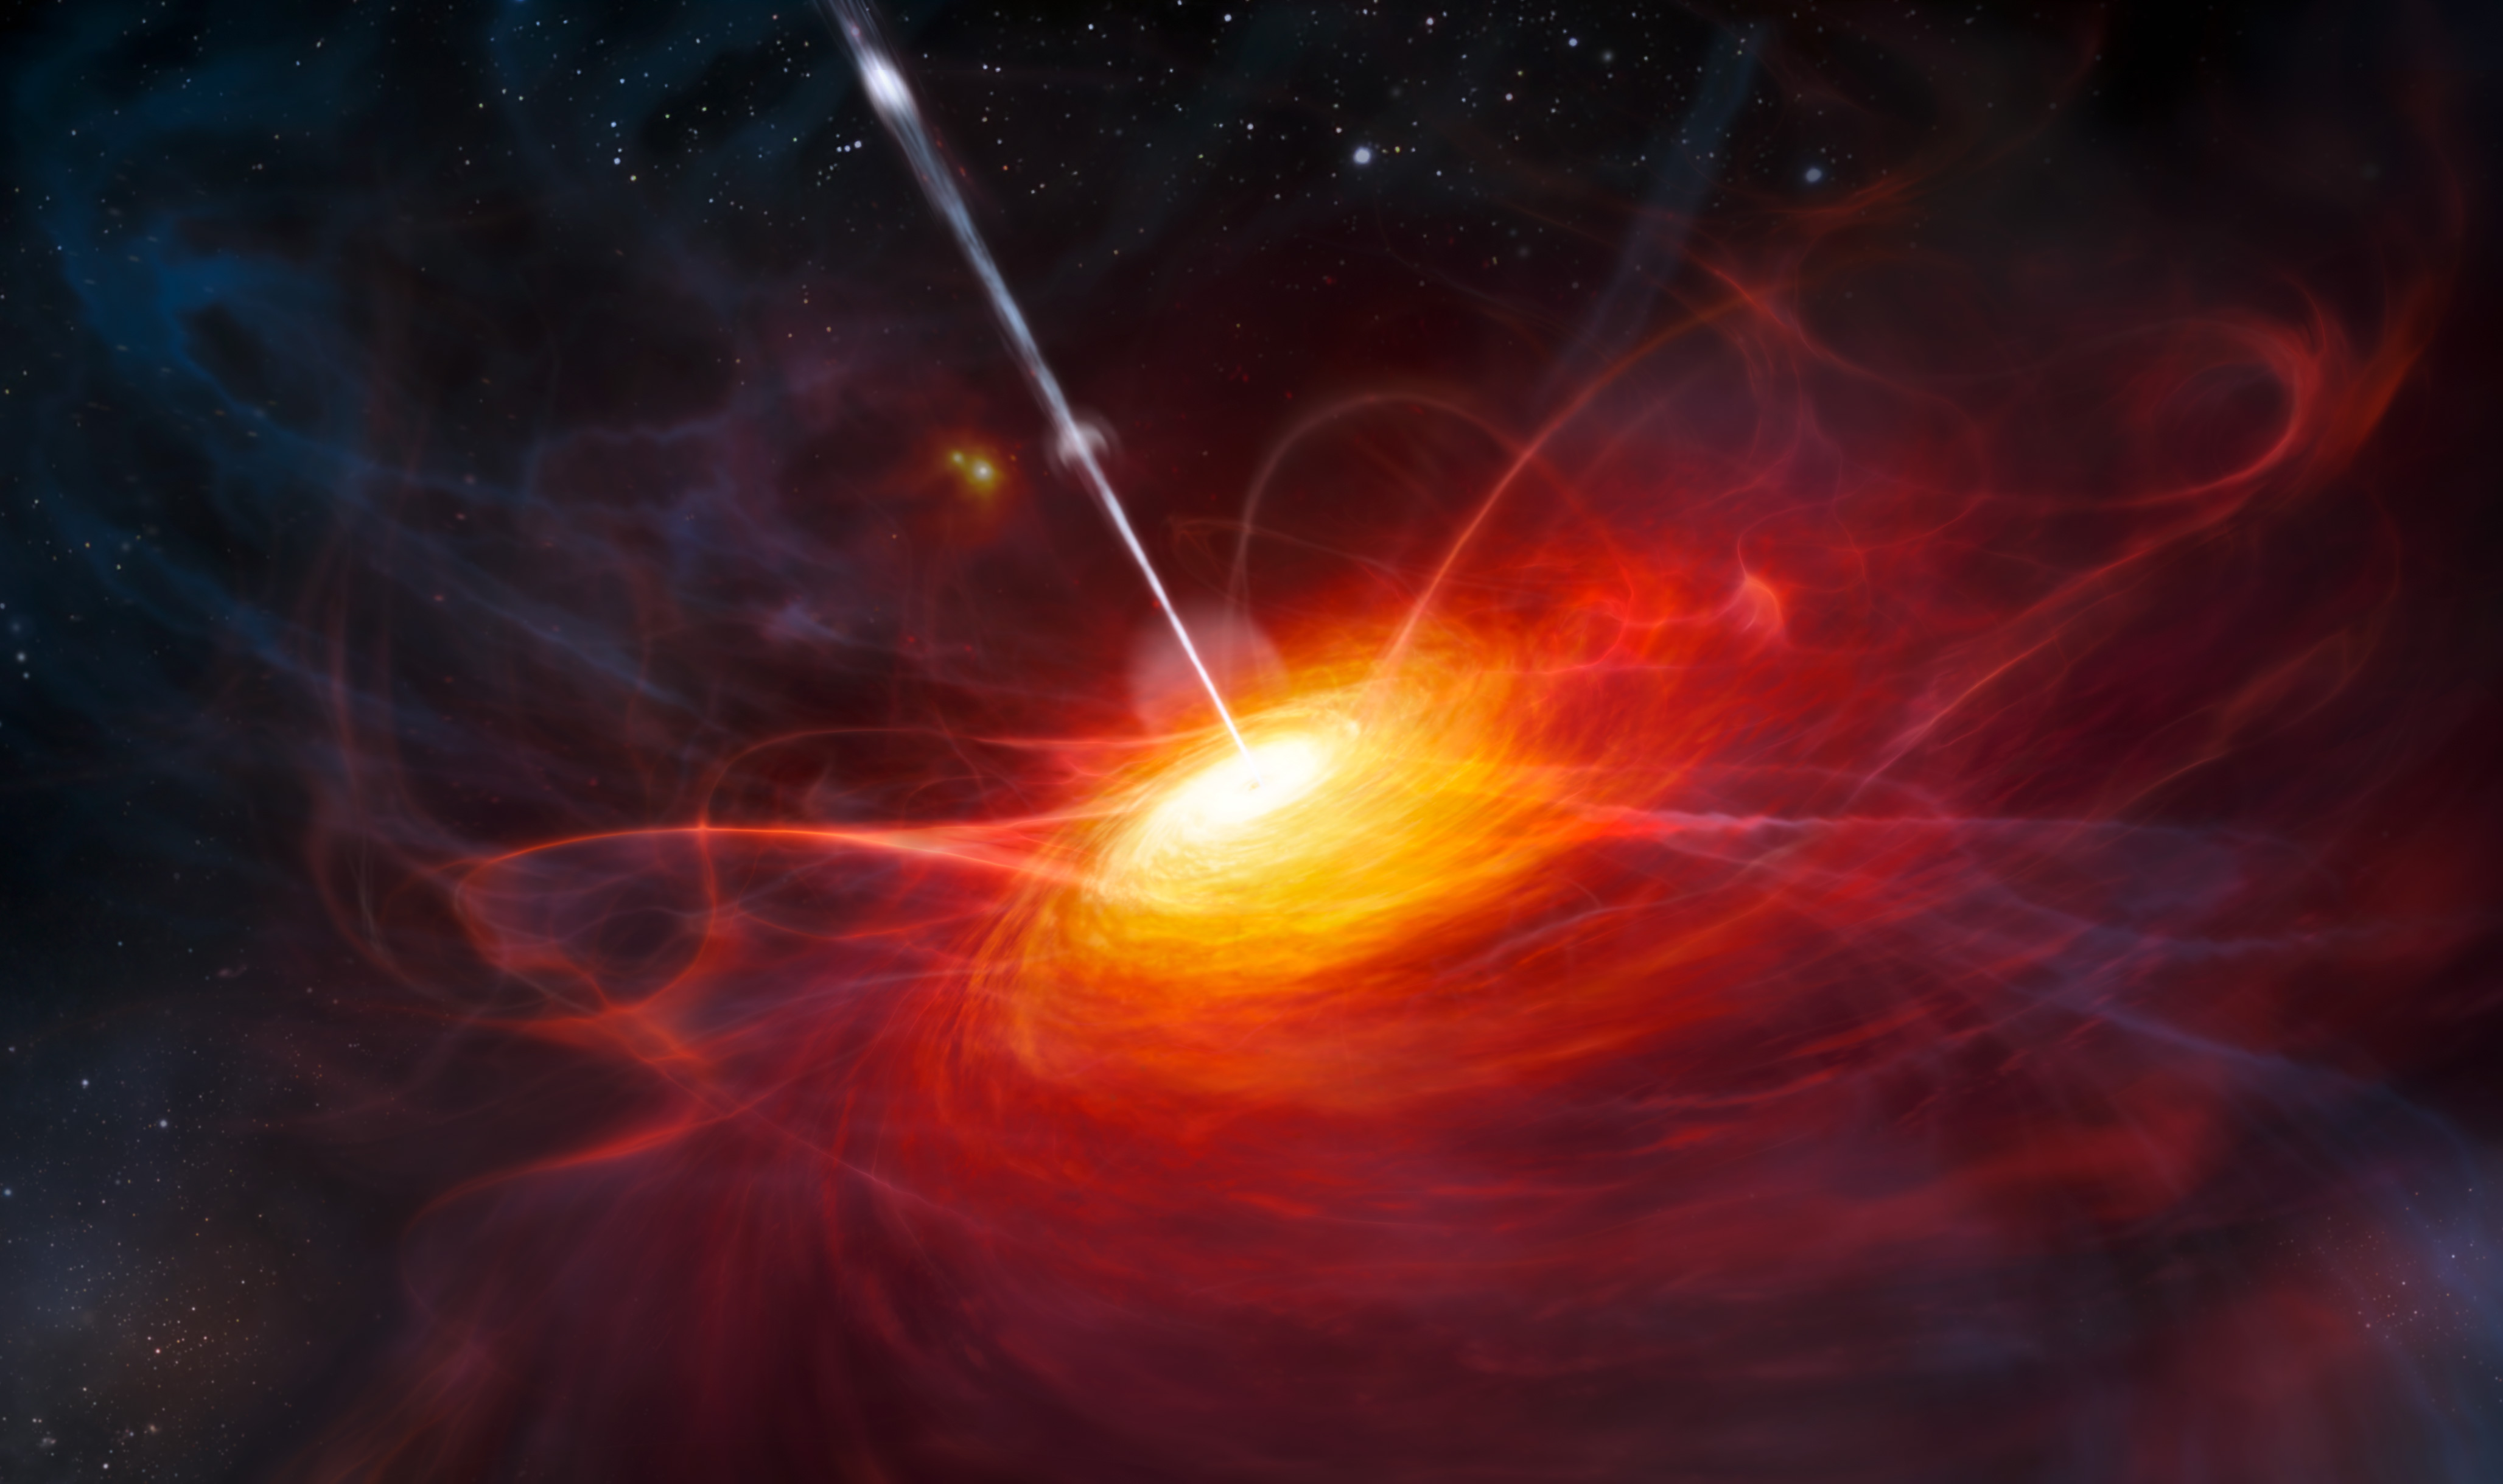
\includegraphics[width=.5\textwidth]{resources/quasar-rendering.jpg}
		\caption{Аккреционный диск квазара ULAS J1120+0641, обнаруженного в 2011 году, в представлении художника.}
	\end{figure}
	Что тогда такое \emph{микроквазары}?

\end{frame}

\begin{frame}
	\frametitle{Некоторые известные микроквазары}
	В 1979 году был открыт экзотический объект \textbf{SS 433}:
	\begin{figure}[h]
		\begin{subfigure}{0.4\textwidth}
			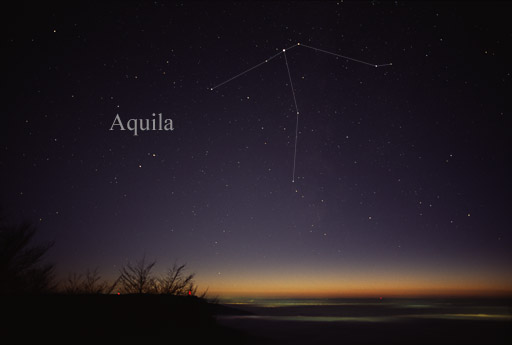
\includegraphics[width=.9\linewidth]{resources/AquilaCC.jpg}
			\caption{Созвездие Орёл}
		\end{subfigure}
		\begin{subfigure}{0.4\textwidth}
			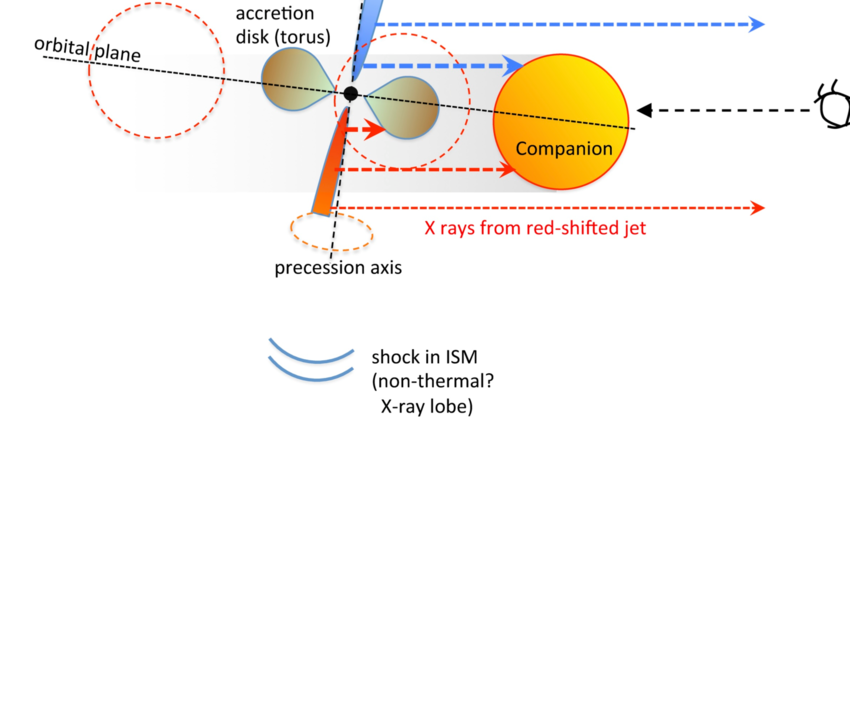
\includegraphics[width=.5\textwidth]{resources/ss-433-schematic-view.png}
			\caption{Схематическое изображение SS 433, Hirofumi Noda}
		\end{subfigure}

		\caption{Объект SS 433}
	\end{figure}

\end{frame}

\begin{frame}
	\frametitle{Как это выглядит (в рентгеновском диапазоне)?}
	Тут должно быть про то, как микроквазары излучают.
\end{frame}



\end{document}
